\section{Реализация Tree RCU}\label{sec:tree_rcu}

Основное преимущество RCU заключается в том, что он позволяет
ожидать выхода весьма большого числа потоков-читателей из своих
критических секций без необходимости учета каждого из них:
в ядрах с non-preemptible реализацией многопоточности их число
ограничено количеством ядер процессора,
в ядрах с preemptible реализацией --- неограниченно вовсе.
Несмотря на то, что примитивы чтения RCU обладают замечательными
показателями производительности и масштабируемости,
примитивы записи должны оттягивать фазу освобождения до тех пор,
пока все потоки-читатели не выйдут из своих критических секций,
за счет блокирования или регистрации callback'а, который должен быть
вызван по истечении grace-периода.
Производительность и масштабируемость RCU определяются
эффективности механизмов обнаружения окончания \emph{grace}-периода.
Например, простейшая реализация RCU может требовать,
чтобы каждое ядро процессора использовало глобальную блокировку
для каждого grace-периода, но этот подход существенно снизит
производительность и масштабируемость.
Для реальных систем, имеющих тысячи процессоров и управляемых Linux,
данный подход неприменим. Этот факт послужил причиной создания Tree RCU.

\subsection{Обзор}
% Lihao: include this in PhD thesis; also look for 'preemptible RCU contents'
%There are several flavors of RCU, including RCU-sched, RCU-preempt,
%RCU Bot\-tom-Half, and Sleepable RCU (SRCU)~\cite{MckenneyRCUflavors}.
% Different flavors have different quiescent states, which are
% discussed in Section \ref{sec:quiescent_state}.
%
% Classic RCU has two implementations: Tiny RCU and Tree RCU. Tiny RCU
% is only for uni-processor systems; we therefore focus on Tree RCU in this paper.
% Tree RCU further has non-pre\-emptible and preemptible variants,
% configured by the kernel Kconfig option \co{CONFIG_PREEMPT}.
% There is no preemptible implementation of Tiny RCU: Instead,
% preemptible Tree RCU is used in single-CPU preemptible kernel builds.
%
% Tree RCU implements RCU-sched, RCU-bh, and RCU-preempt when \co{CONFIG_PREEMPT=y}.
% If \co{CONFIG_PREEMPT=n}, then RCU-preempt is mapped into RCU-sched.
% Tiny RCU requires \co{CONFIG_PREEMPT=n}, so it also maps
% RCU-preempt into RCU-sched.
%
Будем рассматривать <<стандартный>> программный интерфейс RCU
в комбинации с non-preemptible версией ядра Linux,
концентрируясь в основном на примитивах
\co{rcu_read_lock()}, \co{rcu_read_unlock()} и \co{synchronize_rcu()}.
%
%\comment{Lihao: it seems the Tree implementation of Classic RCU also
%implements other three flavors: RCU-sched, RCU-bh, and RCU-preempt;
%and Tiny RCU implements RCU-sched and RCU-bh. Am I right?
%Conceptually, what is the relationship between flavors Classic RCU and
%RCU-sched/RCU-bh? I shall discuss their relationship here otherwise
%readers may get confused when we discuss different flavors in the
%Tree RCU implementation in later sections.}
%\comment{Paul:
%	Yes, Tree RCU implements RCU-sched, RCU-bh, and RCU-preempt,
%	but only when \co{CONFIG_PREEMPT=y}.
%	If \co{CONFIG_PREEMPT=n}, then RCU-preempt is mapped into
%	RCU-sched.
%	Because Tiny RCU is requires \co{CONFIG_PREEMPT=n}, it behaves
%	the same as does Tree RCU when \co{CONFIG_PREEMPT=n},
%	implementing RCU-sched and RCU-bh, and mapping RCU-preempt into
%	RCU-sched.
%	For RCU-preempt, any location outside of an RCU read-side
%	critical section is a quiescent state.
%	For RCU-sched, context switch, idle, userspace,
%	\co{cond_resched_rcu_qs()}, and offline are all quiescent
%	states.
%	For RCU-bh, any location where bottom-half execution is enabled
%	is a quiescent state.
%	Use RCU-sched when you need updaters to wait on hardware interrupt
%	handlers (device drivers) or preempt-disable regions (tracing).
%	Use RCU-bh when networking denial-of-service attacks are a potential
%	issue.}
%
% In a non-pre\-empt\-ible kernel, Tiny and Tree RCU use the same
% \co{rcu_read_lock()} and \co{rcu_read_unlock()} implementation.
% Tiny RCU's \co{synchronize_rcu()} implementation is trivial,
% while preemptible and non-pre\-emptible Tree RCU largely share a rather
% elaborate implementation.
%
Основная идея заключается в том, что примитивы чтения RCU являются
частью ядра и поэтому в его non-preemptible конфигурациях не блокируются.
Поэтому каждый раз, когда ядро процессора простаивает в состоянии бездействия
или блокируется в процессе выполнения пользовательских программ,
все критические секции чтения RCU, запущенные ранее на этом ядре,
оказываются завершенными.
Поэтому каждое из этих состояний называется \emph{устойчивым состоянием}.
Каждый такой переход через устойчивое состояние сигнализирует об
окончании соответствующего grace-периода.
%\comment{Paul: Shouldn't the definition of quiescent state be before the
%first use?}
%\comment{Lihao: move here from the Read-Side Primitives subsection}
% \comment{Lihao: add an overview and high-level idea of how the implementation of Tree RCU works.}
Основная сложность заключается в том, чтобы определить момент,
когда все необходимые устойчивые состояния были пройлены для данного
grace-периода, сохранив при этом высокую производительность и масштабируемость.

Например, использование единой структуры данных для регистрации устойчивых
состояний каждого ядра приводит к неприемлемо частому использованию
блокировок на крупных системах, что в свою очередь приводит к снижению
производительности.
Для решения этой проблемы Tree RCU использует иерархическую организацию
структур данных, каждый узел которой предназначен для учета устойчивых
состояний отдельного ядра и предоставляет свою информацию более высоким уровням.
По достижении корня дерева grace-период заканчивается и
его информация распространяется по всем узлам-потомкам.
Вскоре после того, как узлы получают данную информацию,
происходит возврат из \co{synchronize_rcu()}.

В оставшейся части данного раздела мы рассмотрим реализацию Tree RCU
в non-preemptible конфигурации ядра Linux версии 4.3.6.
Вначале мы вкратце опишем реализацию примитивов чтения и записи,
затем опишем иерархическую структуру данных, используемую для эффективного
учета устойчивых состояния, и, наконец, рассмотрим, как RCU использует
эту структуру данных для фиксации устойчивых состояний и grace-периодов
без учета отдельных потоков-читателей.

%\subsection{Read-Side Primitives} \label{sec:read_api_impl}
\subsection{Read/Write-Side Primitives} \label{sec:api_impl}
% Change in recent kernels.
В non-preemptible версии ядра любая область его исходного кода,
которая не использует добровольных блокировок, является неявной
критической секцией чтения RCU. В связи с этим, реализации
\co{rcu_read_lock()} и \co{rcu_read_unlock()} не должны выполнять
никакой работы. Действительно, в production сборках ядра
с выключенным режимом отладки, эта пара примитивов является
пустышками.

В общем случае, когда используется несколько вычислительных ядер процессора,
примитив записи \co{synchronize_rcu()} вызывает \co{wait_rcu_gp()},
которая является внутренней функцией, использующей механизм callback'ов
для отложенного вызова \co{wakeme_after_rcu()} по окончании некоторого grace-периода.
Как подсказывает название, данная функция повторно предназначена для повторного вызова
\co{wait_rcu_gp()}, которая на этот раз ничего не делает,
тем самым позволяя \co{synchronize_rcu()} вернуть управление в вызывающий поток.

%\comment{Lihao: comment out the following preemptible RCU contents if we need space.}
%In a preemptible kernel, \co{synchronize_rcu()} is implemented in
%\co{kernel/rcu/tree_plugin.h}. It first checks whether the variable
%\co{rcu_scheduler_active} is zero. If so, the system is so early in boot
%that there is only one non-preemptible task, again meaning that grace
%periods complete instantaneously, allowing an immediate return.
%Otherwise, if the grace period should be expedited,
%\co{synchronize_rcu_expedited()} is invoked.
%Otherwise, it passes \co{call_rcu()} to \co{wait_rcu_gp()}, which
%registers callback \co{wakeme_after_rcu()}, similar to
%the non-preemptible kernel discussed above.
%%\comment{Lihao: the source code comments state that \co{rcu_scheduler_active = 0}
%%allows RCU to optimize \co{synchronize_sched()} to a simple \co{barrier()}.
%%Where is the code that does this?}
%%\comment{Paul: The comment is incorrect.
%%The \co{synchronize_sched()} function instead checks the number of
%%online CPUs.
%%I have queued a patch with your
%%Reported-by changing the comment's \co{synchronize_sched()} to
%%\co{synchronize_rcu()}.}
%
%RCU's callback handling and grace period detection are explained in Sections
%\ref{sec:rcu_data} and \ref{sec:grace_period}, respectively.

% Lihao: understand how call_rcu_sched works and understand the differences from
% the Tiny RCU version which only calls the kernel function cond_resched()
%
% Lihao: In a preemptible kernel, the implementation of \co{synchronize_rcu()}
% http://lxr.free-electrons.com/source/kernel/rcu/tree_plugin.h#L539 and
% understand the differences between preemptible and non-preemptible versions

\subsection{Структуры данных Tree RCU} \label{sec:data_structure}

\begin{figure}[tbp]
\centering
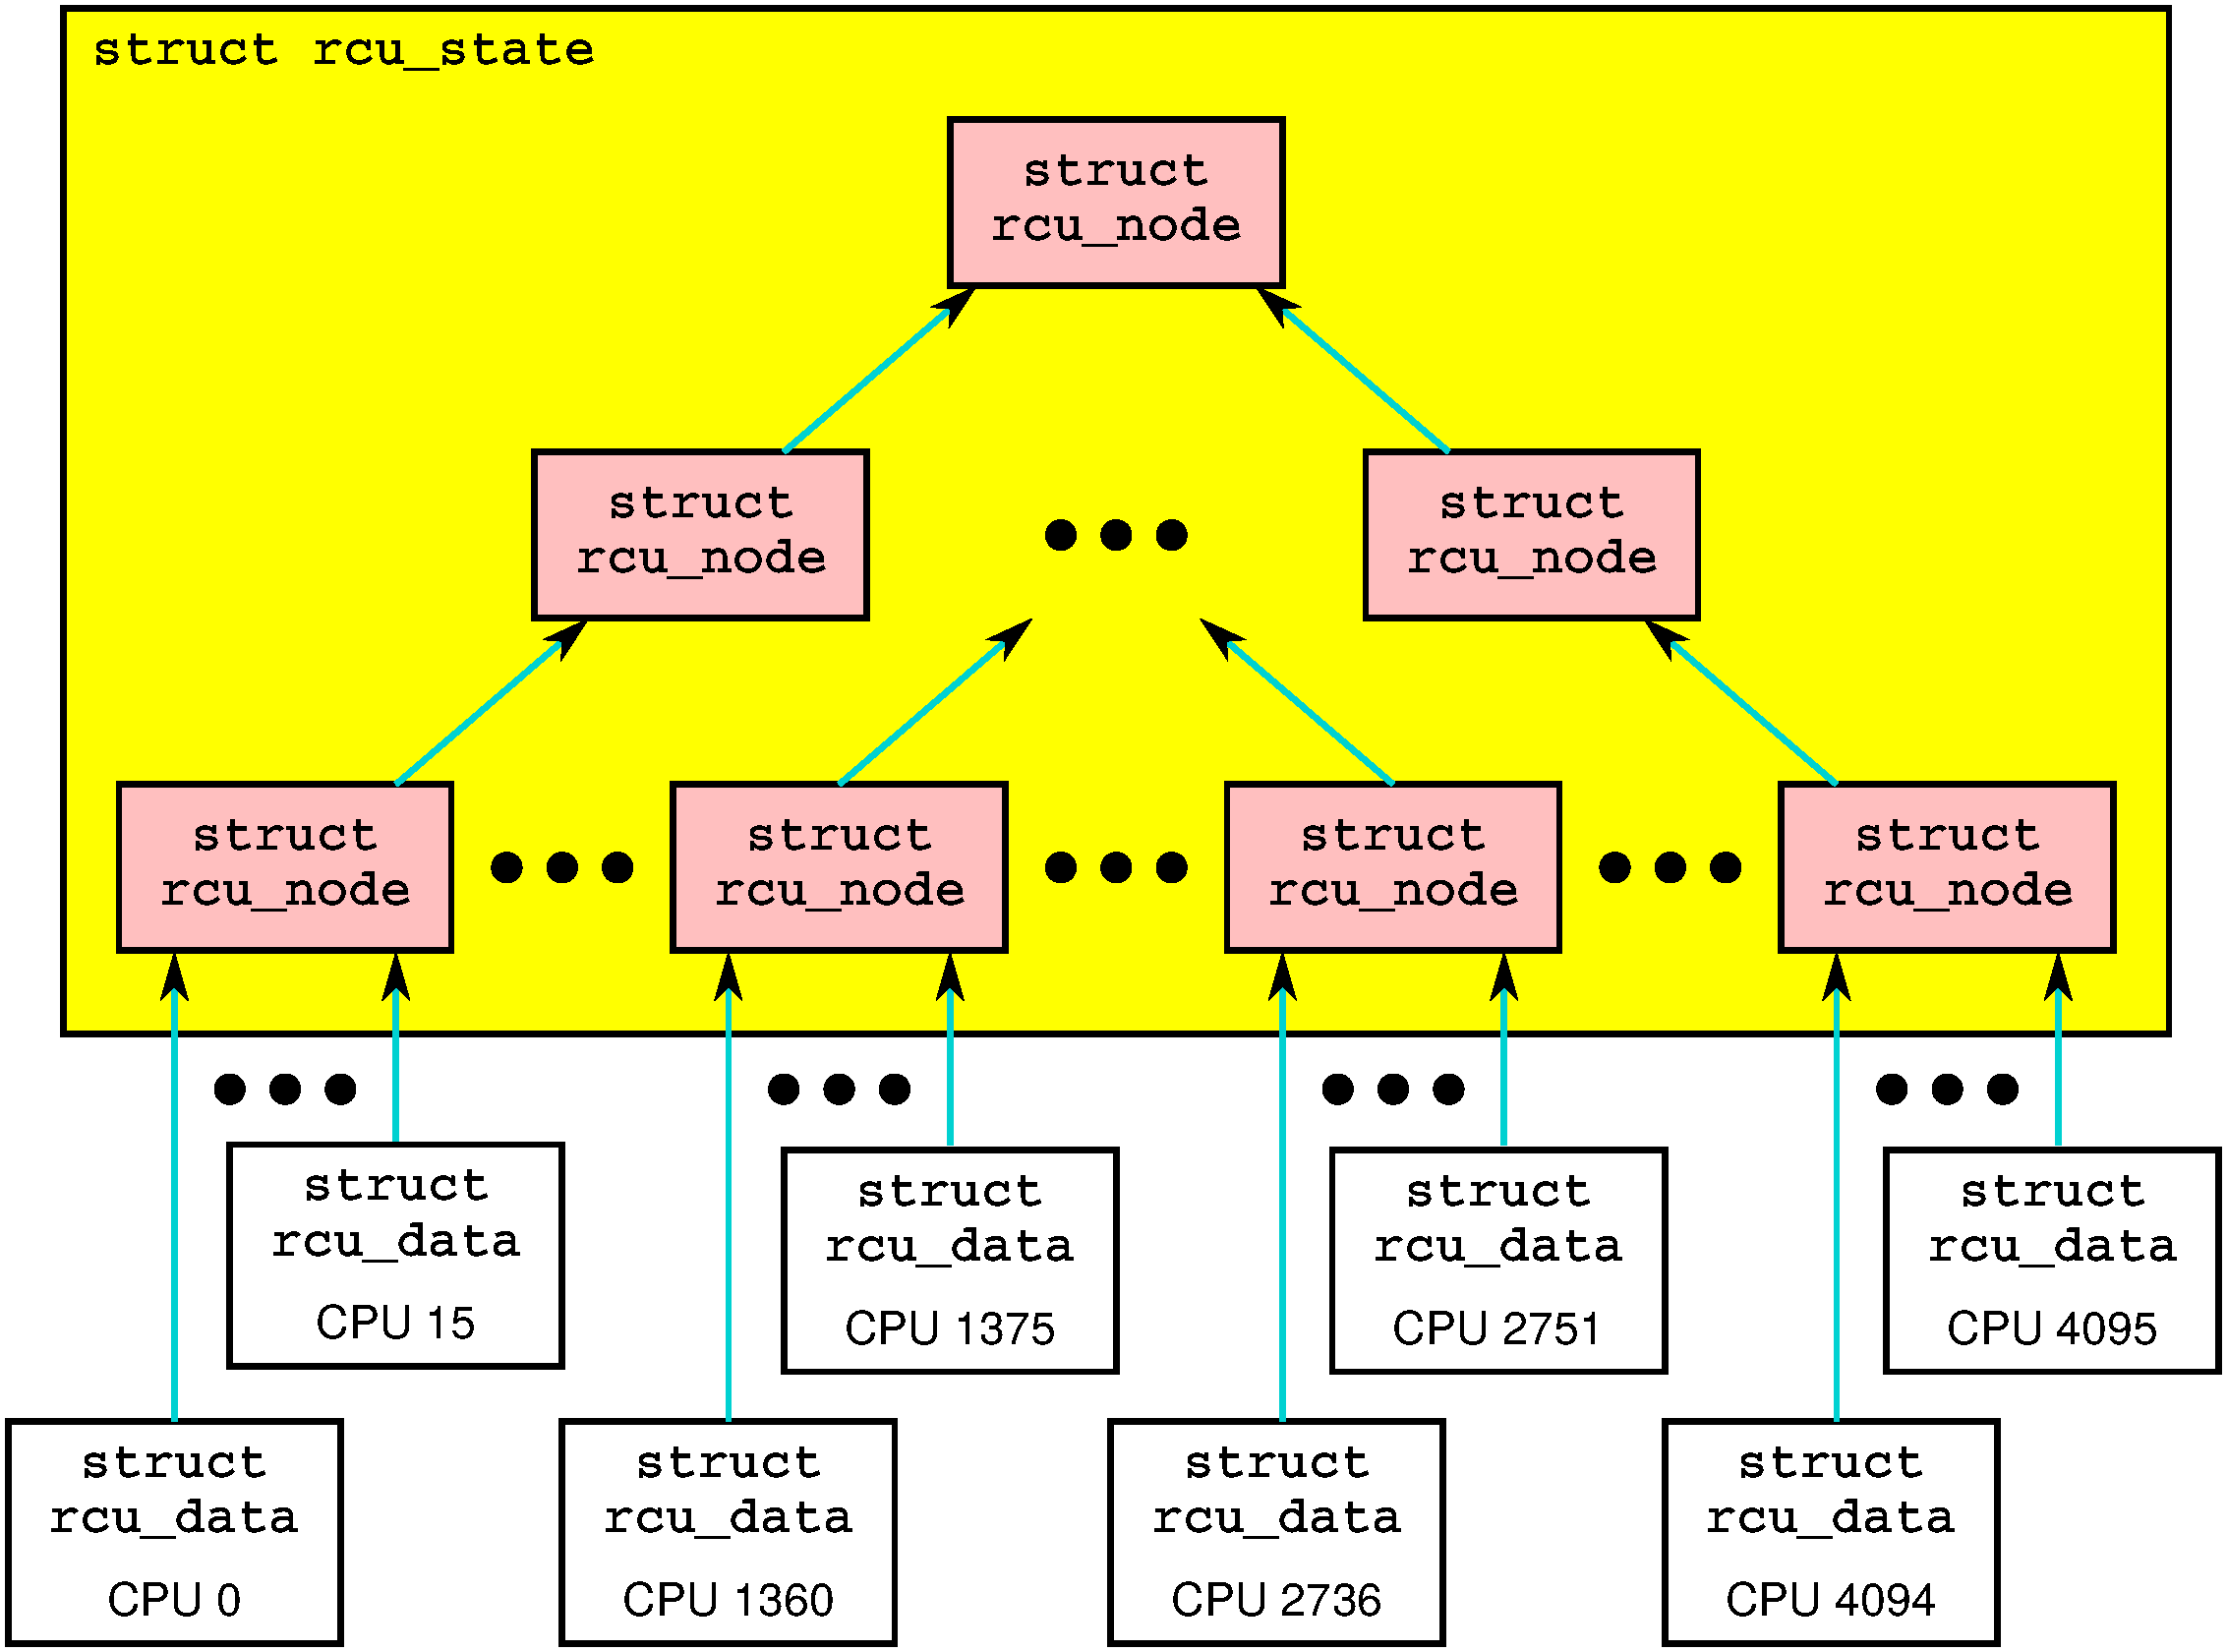
\includegraphics[scale=0.2]{tree_rcu_hierarchy.pdf}
\caption{Иерархия Tree RCU}
\label{fig:tree_rcu_hierarchy}
\end{figure}

Глобальное состояние RCU записывается в структуру \co{rcu_state},
представляющую собой дерево структур \co{rcu_node} с арностью, равной 64
(32 на 32-битных системах). Каждый терминальный узел данного дерева
может иметь ссылки на максимум 64 (32 на 32-битных системах) структуры
\co{rcu_data} каждая из которых соответствует отдельному ядру процессора,
как показано на рисунке~\ref{fig:tree_rcu_hierarchy}.
Каждая структура \co{rcu_data} ведет учет устойчивых состояний своего ядра,
а \co{rcu_node}-дерево используется сначала для распространения информации
об этих состояниях в направлении корня,
а затем --- для распространия информации о grace-периодах в направлении листьев.
Информация об устойчивых состояниях передается на родительский уровень
в тот момент времени, когда каждый узел-потомок каждого поддерева данного уровня
уже передал её в корень этого поддерева.
Эта схема передачи информации позволяет существенно сократить частоту использования
блокировок на верхних уровнях дерева.
Например, рассмотрим стандартное \co{rcu_node} дерево для системы с
4{,}096 вычислительными ядрами, имеющее 256 терминальных узлов,
4 внутренних узлов и один корневой узел. В течение данного grace-периода,
каждое ядро процессора сообщит информацию о своем устойчивом состоянии в
соответствующий терминальный узел, но при этом каждому терминальному узлу
будет соответствовать всего 16 соперничающих ядер.
Всего 256 ядер будут пытаться сообщить свои устойчивые состояния внутренним узлам,
при этом всего информация 64 ядер дойдет до каждого из четырех внутренних узов.
Наконец, информация всего четырех ядер может дойти до корневого узла,
что приводит к очень низкой частоте его блокирования.
Это позволяет использовать данную структуру на очень больших системах.
В частности, существующая реализация RCU ядра Linux поддерживает
четырехуровневые деревья, что позволяет использовать до
$64^4 = 16{,}777{,}216$ ядрами на 64-битных системах.\footnote{
  В настоящее время четырехуровневые деревья используются при нагрузочном тестировании,
  а трехуровневые находят свое применение на промышленных 4096-ядерных системах.}

\subsubsection{Структура \co{rcu_state}}

\begin{figure}[tbp]
\centering
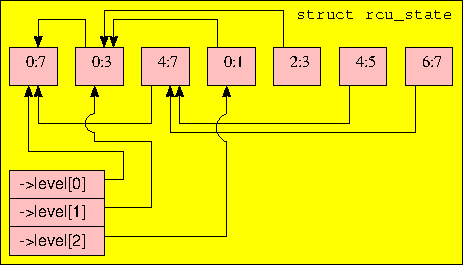
\includegraphics[scale=0.9]{rcu_node_array.pdf}
\caption{Представление дерева структур \co{rcu_node} в виде массива}
\label{fig:rcu_node_array}
\end{figure}

Каждая реализация RCU имеет свою собственную структуру \co{rcu_state}.
Структура \co{rcu_state} включает в себя массив структур \co{rcu_node},
логически организованных в виде дерева \co{struct rcu_node node[NUM_RCU_NODES]},
со структурами \co{rcu_data}, присоединенными к его терминальным узлам.
Таким образом, обход этого дерева в ширину сводится к линейному проходу по массиву.
Еще один массив структур \co{rcu_node}, \co{*level[NUM_RCU_LVLS]},
используется для указания на самый левый узел каждого уровня дерева,
как показано на рисунке~\ref{fig:rcu_node_array}.

Структура \co{rcu_state} использует поля \co{->gpnum} и \co{->completed}
типа \co{unsigned long} для учета grace-периодов.
Поле \co{->gpnum} используется для отслеживания начала последнего grace-периода,
в то время как \co{->completed} отслеживает окончание последнего grace-периода.
Если значения данных полей одинаковы, то RCU находится в состоянии по умолчанию.
Если же значение \co{gpnum} больше, чем \co{completed}, то RCU находится в состоянии
grace-периода. Все прочие комбинации являюется недопустимыми.

\subsubsection{Структура \co{rcu_node}}
\label{sec:rcu_node}
Дерево структур \co{rcu_node} регистрирует и распространяет
информацию об устойчивых состояниях от терминальных узлов к корневому,
а также распространяет информацию о grace-периодах в обратном направлении.
Структура \co{rcu_node} использует спин-блокировку \co{->lock} для защиты
своих полей. Поле \co{->parent} содержит указатель на струтуру-родителя,
при этом значение данного поля у корневого узла равно \co{NULL}.
Значение поля \co{->level} равно номеру уровня,
на котором находится данный узел в дереве,
считая уровень корневого узла нулевыми.
Поле \co{->grpmask} описывает номер бита данного узла в значении поля
\co{->qsmask} узла-родителя.
Поля \co{->grplo} и \co{->grphi} соответствуют наименьшему и наибольшему
порядковому номеру вычислительного ядра, учитываемого данной структурой.

Поле \co{->qsmask} указывает, какие из узлов-потомков еще не сообщили
о своих устойчивых состояниях на данный момент времени.
Как и в случае с \co{rcu_state}, структура \co{rcu_node} имеет поля
\co{->completed} и \co{->gpnum}, имеющие такие же значения, как и у родительской
структуры \co{rcu_state}, за исключением начала и конца каждого
grace-периода, когда данные значения копируются из корневого узла.
Значения этих полей могут быть равны друг другу, либо отличаться на единицу.

\subsubsection{Структура \co{rcu_data}} \label{sec:rcu_data}
Структурв \co{rcu_data} используется для учета устойчивых состояний и
вызова callback'ов связанного вычислительного ядра.
Поскольку доступ к данной структуре только осуществляется посредством
связанного вычислительного ядра, нет необходимости выполнять синхронизацию.
Как и в случае со структурой \co{rcu_state}, различные реализации RCU поддерживают
различные виды структур \co{rcu_data}.
Поле \co{->cpu} указывает на связанное вычислительное ядро,
\co{->rsp} --- на связанную структуру \co{rcu_state},
а \co{->mynode} ссылается на соответсвующую терминальную структуру \co{rcu_node}.
Значение поля \co{->grpmask} указывает на позицию структуры \co{rcu_data}
в битовом поле \co{->qsmask} связанной структуры \co{rcu_node}.

Структура \co{rcu_data} содержит поле \co{->qs_pending}, указывающее,
что RCU ожидает получения устойчивого состояния от связанного ядра,
и поле \co{->passed_quiesce}, указывающее на то, что данное ядро уже
прошло через устойчивое состояние.
Кроме этого, данная структура имеет поля \co{->gpnum} и \co{->completed},
значения которых могут отставать от соответсвующих им полей структур
\co{rcu_state} и \co{rcu_node} в режиме простоя ядер процессора.
С другой стороны, если ядра процессора являются заблокированными,
их значения могут оставать лишь на один grace-период от соответсвующих значений
полей структуры \co{rcu_node}.

Поля \co{->gpnum} и \co{->completed} структуры \co{rcu_state} содержат наиболее
актуальные значения и используются для обновления соответствующих полей родительских
структур \co{rcu_node}, что позволяет сравнивать значения данных полей со значениями
этих же полей структур \co{rcu_node} для фиксации факта начала очередного grace-периода.
Эта схема позволяет вычислительным ядрам обнаруживать границы grace-периодов
без использования блокировок.
Структруа \co{rcu_data} управляет RCU callback'ами с помощью
структуры данных, известной как четырехсегментный
список~\cite{LaiJiangshan2008NewClassicAlgorithm}.

\begin{figure}[tbp]
\centering
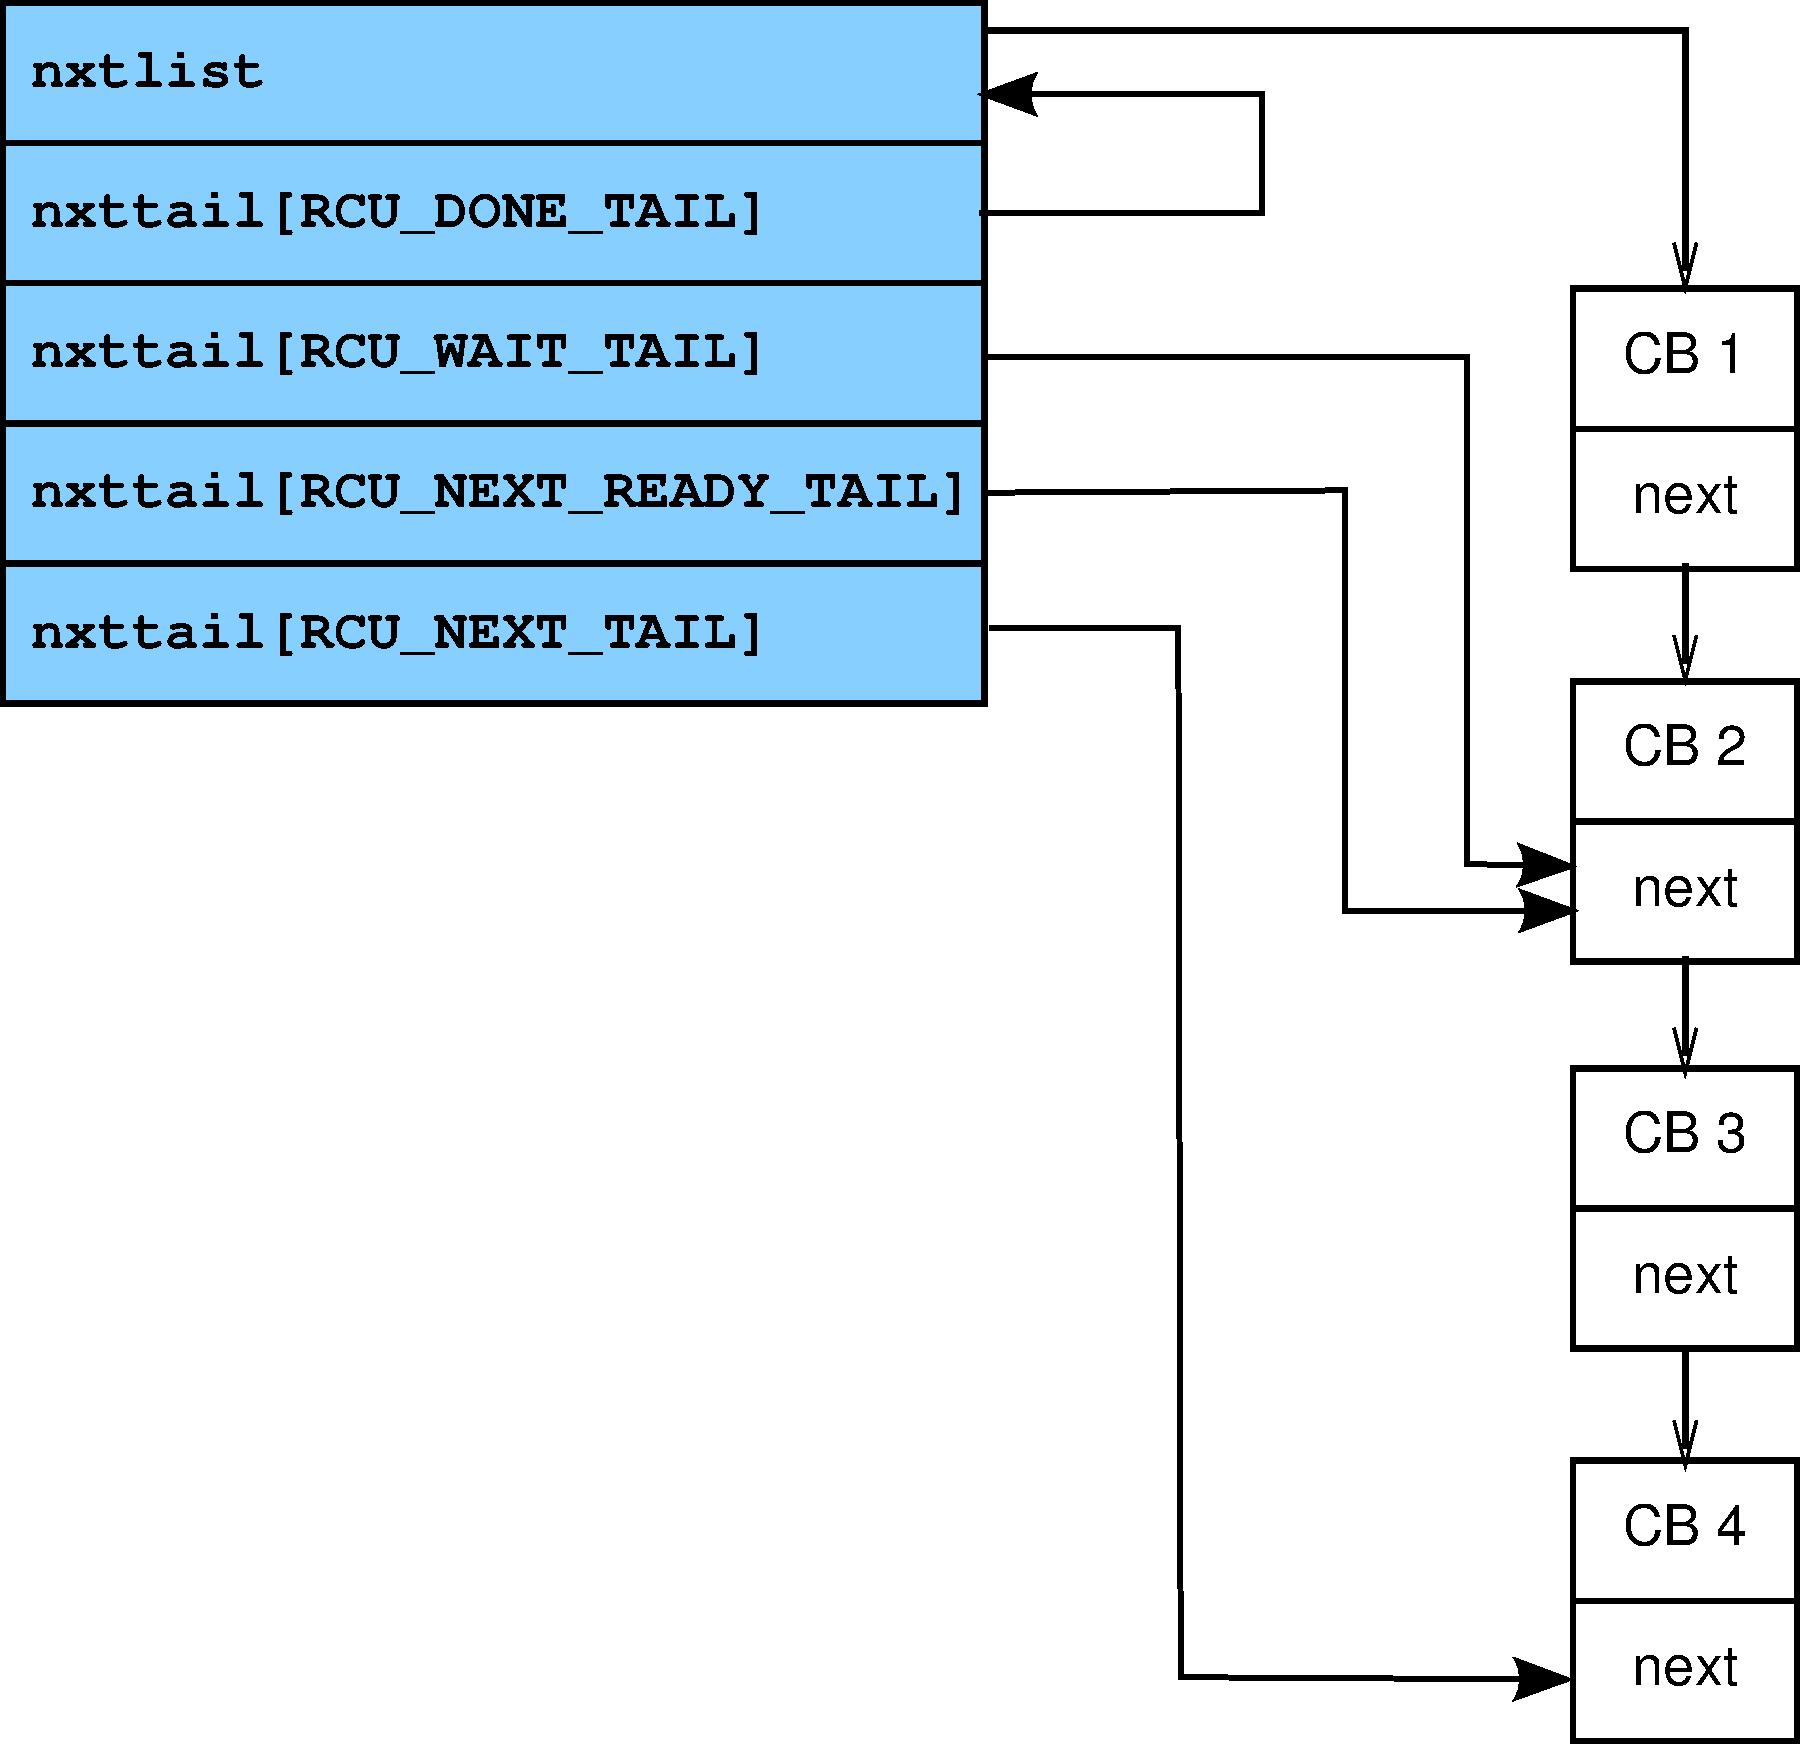
\includegraphics[scale=0.25]{rcu_data_callbacks.pdf}
\caption{Callback Queuing in \co{rcu_data}}
\label{fig:rcu_data_callbacks}
\end{figure}

%\comment{Lihao: since we don't model callbacks, only describe them briefly and add a reference
%to save space for the experiments section which is the main contribution of this paper. 
%Do the same for discussion of preemptible RCU.}
\subsubsection{RCU Callbacks}
The \co{rcu_data} structure manages RCU callbacks using a \co{->nxtlist}
pointer tracking the head of the list and an array of \co{->nxttail[]}
tail pointers that form a four-segment list of
callbacks~\cite{LaiJiangshan2008NewClassicAlgorithm}, with
each element of the \co{->nxttail[]} array referencing the tail of the
corresponding segment, as shown in Figure~\ref{fig:rcu_data_callbacks}.
The segment ending with \co{->nxttail[RCU_DONE_TAIL]} (the ``\co{RCU_DONE_TAIL}
segment'') contains callbacks
handled by a prior grace period that are therefore ready to be invoked.
The \co{RCU_WAIT_TAIL} and \co{RCU_NEXT_READY_TAIL} segments 
contain callbacks waiting for the
current and the next grace period, respectively.
Finally, the \co{RCU_NEXT_TAIL} segment contains
callbacks that are not yet associated with any grace period.
%
The \co{->qlen} field counts the total number of callbacks, and
the \co{->blimit} field specifies the maximum number of RCU callbacks
that may be invoked at a given time, thus limiting response-time
degradation due to long lists of callbacks.\footnote{
	Workloads requiring aggressive real-time guarantees should use
	callback offloading, which is outside of the scope of this paper.}

Back in Figure~\ref{fig:rcu_data_callbacks}, the
\co{->nxttail[RCU_DONE_TAIL]} array element references \co{->nxtlist}, 
which means none of the callbacks are ready to invoke.
The \co{->nxttail[RCU_WAIT_TAIL]} element references callback 2's \co{->next}
pointer, meaning that callbacks CB~1 and CB~2 are waiting for the current
grace period.
The \co{->nxttail[RCU_NEXT_READY_TAIL]} element references that same \co{->next}
pointer, meaning that no callbacks are waiting for the next grace period. 
Finally, the callbacks between the \co{->nxttail[RCU_NEXT_READY_TAIL]} and
\co{->nxttail[RCU_NEXT_TAIL]} elements (CB~3 and CB~4)
are not yet assigned to a specific grace period.
The \co{->nxttail[RCU_NEXT_TAIL]} element always references either
the last callback or, when the entire list is empty, \co{->nxtlist}.

Cache locality is promoted by invoking callbacks on the CPU that registered
them.
For example, RCU's update-side primitive 
\co{synchronize_rcu()} appends callback \co{wakeme_after_rcu()} to the end
of the \co{->nxttail[RCU_NEXT_TAIL]} list in the current CPU 
(Section \ref{sec:update_api_impl}). 
They are advanced one segment towards the head of the list (via \co{rcu_advance_cbs()}) 
when the CPU detects the current grace period has ended, which is indicated 
by the \co{->completed} field of the CPU's \co{rcu_data} structure being one
smaller than its counterpart in the corresponding leaf \co{rcu_node} structure.
The CPU also periodically merges the \co{RCU_NEXT_TAIL} segment into the
\co{RCU_NEXT_READY_TAIL} segment by calling \co{rcu_accelerate_cbs()}.
In a few special cases, the CPU merges the \co{RCU_NEXT_TAIL} segment
into the \co{RCU_WAIT_TAIL} segment, bypassing the \co{RCU_NEXT_TAIL}
segment.
This optimization applies when the CPU is starting a new grace period.
It does \emph{not} apply when a CPU notices a new grace period
because that grace period might well have started before
the callbacks were added to the \co{RCU_NEXT_TAIL} segment.
%\comment{Lihao: why can't we invoke *all* callbacks when starting a new 
%grace period? Isn't it true that all pre-existing read-side critical
%sections, i.e.~those start before callbacks are registered in \co{->nxttail} 
%(in particular \co{wakeme_after_rcu} in \co{->nxttail[RCU_NEXT_TAIL]}), 
%have finished?}
%\comment{Paul: In theory, we could, but in practice doing this would
%have several disadvantages:
%(1) All callbacks would be invoked by the grace-period kthread, and
%large systems could generate more callbacks than a single CPU could
%keep up with, which would delay subsequent grace periods and possibly
%even run the system out of memory.
%(2) Running all the callbacks at once could degrade real-time response.
%(3) Running callbacks on a different CPU than the one that registered
%them would decrease locality, increasing cache-miss rates, thus degrading
%performance.
%(4) This would require that atomic instructions be used when registering
%callbacks (as they are for no-CBs CPUs), further degrading performance.
%In addition, we could only invoke callbacks in the \co{RCU_NEXT_TAIL}
%segment, because callbacks in the later segments
%(\co{RCU_NEXT_READY_TAIL}, \co{RCU_WAIT_TAIL}, and
%\co{RCU_DONE_TAIL} might well have been queued \emph{after} the
%recently-completed grace period started.}
%
This is a deliberate design choice: It is more important for the CPUs
to operate independently (thus avoiding contention and synchronization
overhead) than it is to decrease grace-period latencies.
In those rare occasions where low grace-period latency is important,
the \co{synchronize_rcu_expedited()} should be used.
This function has the same semantics as does \co{synchronize_rcu()},
but trades off efficiency optimizations in favor of reduced latency.
% Lihao: this is where the callback of RCU's update API register? 
% Paul: Yes, call_rcu() appends the callback to the end of the current
% CPU's RCU_NEXT_TAIL list.  Ignoring callback offloading for the moment.
% Lihao: we don't model QS forcing and offline CPUs
% Paul: Nor are you modeling callback offloading.  Which is fine, just calling
% it out.  ;-)

Each RCU callbacks is an \co{rcu_head} structure which has a
\co{->next} field that points to the next callback on the list and
a \co{->func} field that references the function to be invoked at the
end of an upcoming grace period.




\subsection{Обнаружение устойчивых состояний} \label{sec:quiescent_state}
Механизм RCU должен ожидать до тех пор,
пока все потоки не выйдут из своих критических секций чтения перед тем,
как можно будет завершить grace-период.
Производительность и масштабируемость RCU
основывается на его способности быстро обнаруживать
устойчивые состояния вычислительных ядер и определять
момент, когда их набралось достаточно, чтобы завершить
grace-период.
Если каждое ядро (или, в случае preemptible-RCU, каждый поток)
прошел через устойчивое состояние, то можно считать,
что grace-период закончился.

В случае использования non-preemptible RCU-sched вида RCU,
устойчивыми состояниями считаются следующие состояния вычислительных ядер:
выполнение инструкций пользовательского пространства,
переключение контекста, режим ожидания и offline-режим.
RCU-sched отслеживает лишь потоки и векторы прерываний,
которые выполняются в данный момент,
поскольку заблокированные и прерванные потоки всегда находятся в
устойчивых состояниях.
Таким образом, RCU-sched достаточно отслеживать состояния вычислительных ядер.

\subsubsection{Таймер прерываний} \label{sec:timer_interrupt}
Функция \co{rcu_check_callbacks()} вызывается из обработчика таймера прерываний,
позволяющего RCU периодически проверять, находится ли данное вычислительное
ядро в пользовательском режиме или в одном из устойчивых состояний.
Если ядро находится в одном из этих состояний,
\co{rcu_check_callbacks()} вызывает \co{rcu_sched_qs()},
который изменяет значение поля \co{rcu_sched_data.passed_quiesce} для
каждого ядра.
Функция \co{rcu_check_callbacks()} вызывает \co{rcu_pending()}
для того, чтобы проверить, является ли последнее событие или данное условие
признаком внимания к данному ядру со стороны RCU.
Если да, то \co{rcu_check_callbacks()} вызывает функцию \co{raise_softirq()},
которая приводит к тому, что \co{rcu_process_callbacks()} будет вызвана,
как только ядро достигнет безопасного состояния
(грубо говоря, когда на ядре будут включены прерывания,
preemption и bottom halves).
Эта функция подробно рассматривается в разделе \ref{sec:grace_period}.

\subsubsection{Управление переключениями контекста} \label{sec:context_switch}
Устойчивые состояния, связанные с переключениями контекста,
учитываются путем вызова функции \co{rcu_note_context_switch()} из
\co{__schedule()}
(и, для поддержки виртуализации,
из \co{rcu_virt_note_context_switch()}).
Функция \co{rcu_note_context_switch()} вызывает \co{rcu_sched_qs()}
для оповещения RCU о переключении контекста, которое является устойчивым
состоянием вычислительного ядро.

\subsection{Grace Period Detection} \label{sec:grace_period}
Once each CPU has passed through a quiescent state, a grace period for RCU
has completed. 
As discussed in Section \ref{sec:data_structure}, Tree-RCU uses a hierarchy 
of \co{rcu_node} structures to manage quiescent state and grace period
information.
Quiescent-state information is passed up the 
tree from the leaf per-CPU \co{rcu_data} structures.
Grace-period information is passed down from the root.
%
%The dyntick-idle mechanisms used for idle CPUs and \co{nohz_full} userspace
%execution are out of scope for this research, as are RCU CPU stall warnings. The focus is instead 
We focus on grace-period detection for busy CPUs, as illustrated
in Figure~\ref{fig:grace_period_state_diagram}.

\begin{figure}[tb]
\centering
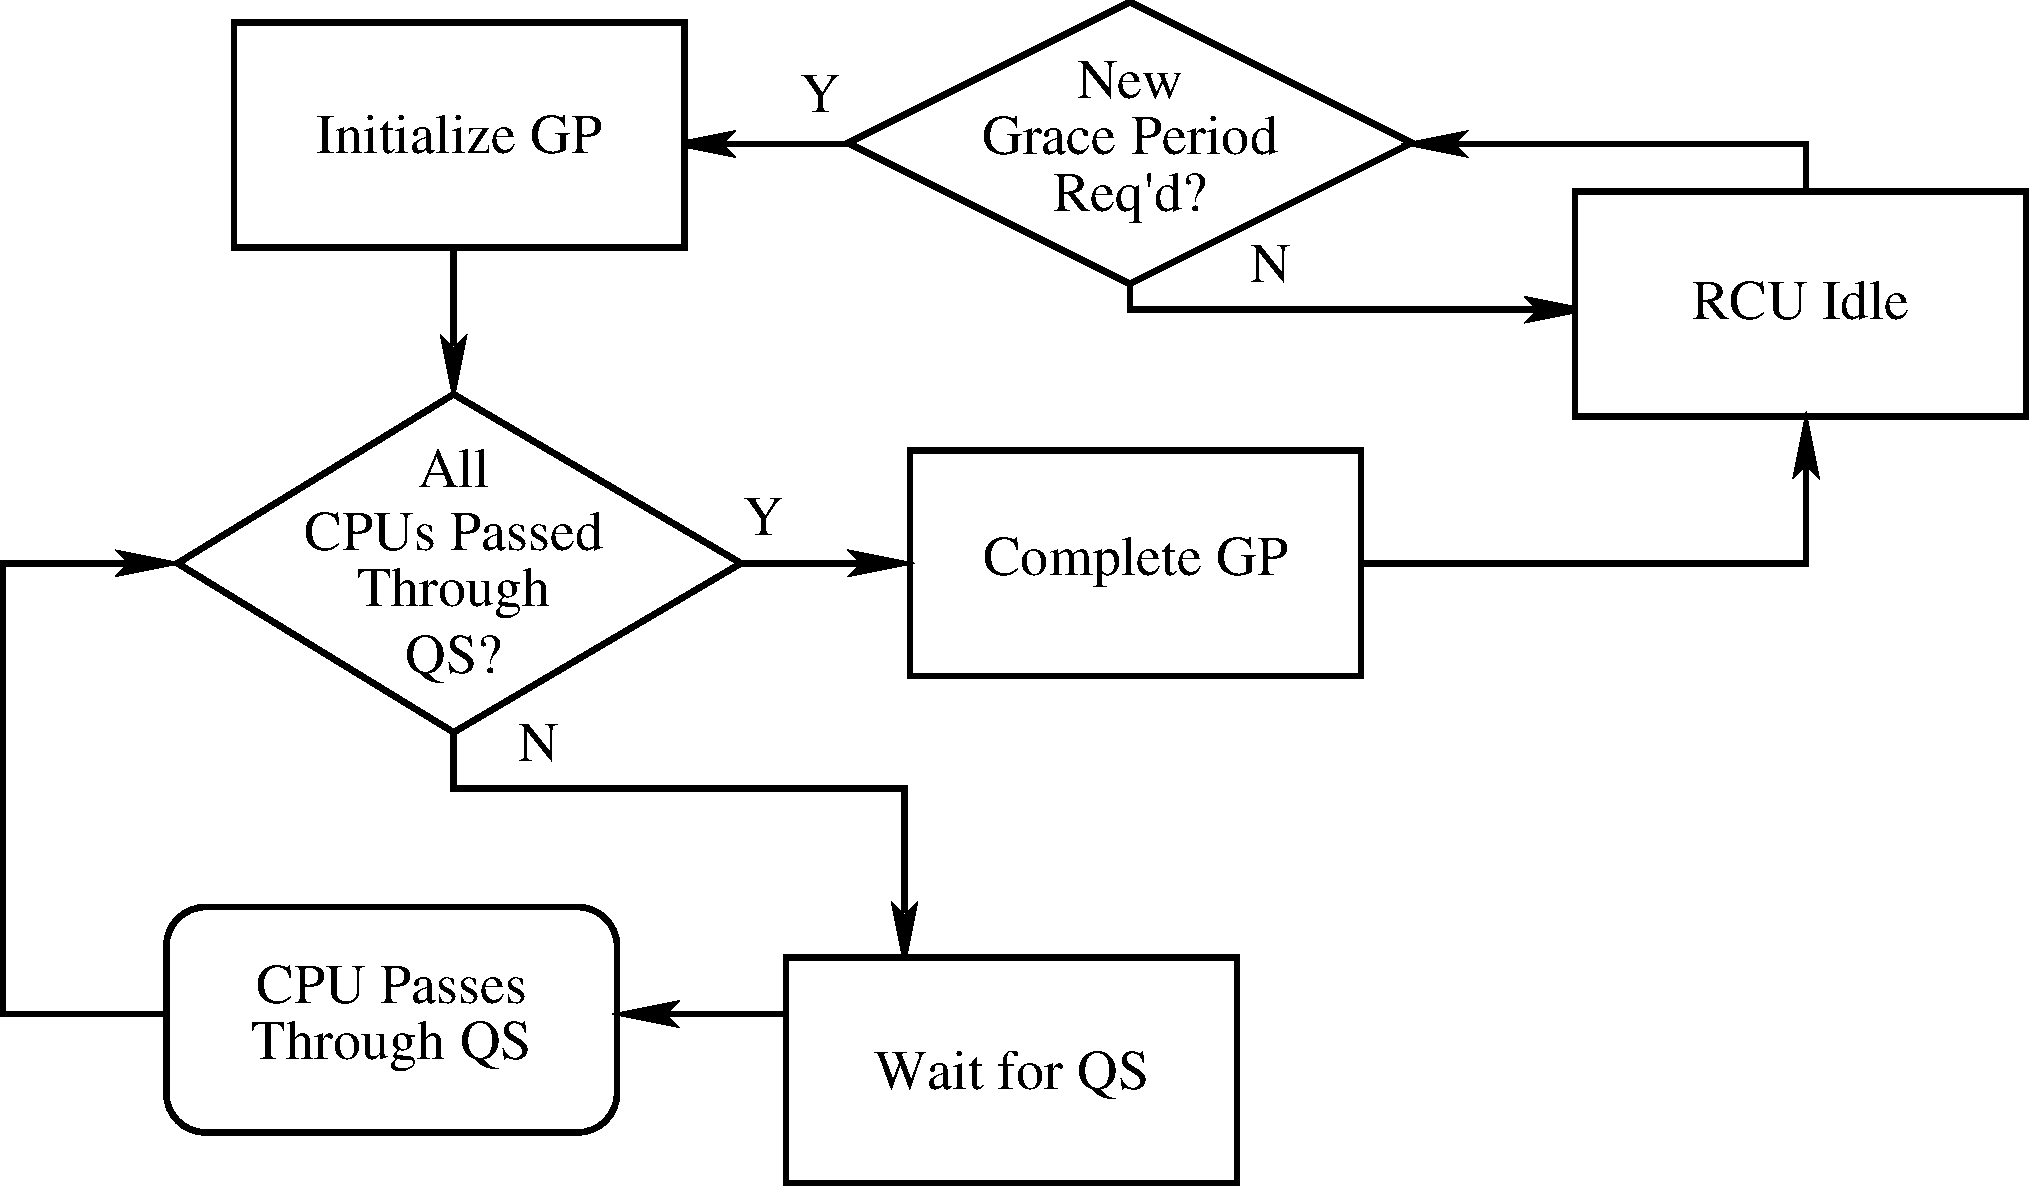
\includegraphics[scale=0.25]{grace_period_state_diagram.pdf}
\caption{Grace-Period Detection State Diagram}
\label{fig:grace_period_state_diagram}
\end{figure}

\subsubsection{Softirq Handler for RCU} \label{sec:rcu_softirq}
RCU's busy-CPU grace period detection relies on the
\co{RCU_SOFTIRQ} handler function \co{rcu_process_callbacks()},
which is scheduled from the scheduling-clock interrupt.
This function first calls
\co{rcu_check_quiescent_state()} to report recent quiescent states
on the current CPU.
Then \co{rcu_process_callbacks()} starts a new grace period if needed,
and finally calls \co{invoke_rcu_callbacks()} to invoke any callbacks
whose grace period has already elapsed.

Function \co{rcu_check_quiescent_state()} first invokes \co{note_gp_changes()} 
to update the CPU-local \co{rcu_data} structure to record the end of 
previous grace periods and the beginning of new grace periods.
%, which are detected via differences in the \co{->completed} and
%\co{->gpnum} fields, respectively.
Any new values for these fields are copied from the leaf \co{rcu_node}
structure to the \co{rcu_data} structure.
If an old grace period has ended, \co{rcu_advance_cbs()} is invoked to
advance all callbacks, otherwise, \co{rcu_accelerate_cbs()} is invoked
to assign a grace period to any recently arrived callbacks.
If a new grace period has started, \co{->passed_quiesce} is set to zero,
and if in addition RCU is waiting for a quiescent state from this CPU,
\co{->qs_pending} is set to one, so that a new quiescent state will
be detected for the new grace period.
%
% Lihao: this is one of the two places where qs_pending gets updated in Tree RCU
% \comment{(Lihao: does it mean even this softirq is invoked because of a quiescent state of this CPU
%   (\co{rdp->passed_quiesce} is set to 1 in \co{rcu_check_callbacks} so \co{rcu_pending} 
%   return 1), if for some reason gpnum in \co{rcu_data} of this CPU is one lag behind its parent 
%   counterpart, this CPU needs to wait for its next quiescent to commit? 
%   \url{http://lxr.free-electrons.com/source/kernel/rcu/tree.c#L1747}
% )}
% Paul: Yes.  I did look into immediately detecting quiescent states for
% RCU-preempt, but it didn't seem worth the coding contortions required.

Next,
\co{rcu_check_quiescent_state()} checks whether \co{->qs_pending} indicates
that RCU needs a quiescent state from this CPU.
If so, it checks whether \co{->passed_quiesce} indicates that this
CPU has in fact passed through a quiescent state.
If so, it invokes \co{rcu_report_qs_rdp()} to report that quiescent
state up the %\co{rcu_data} and \co{rcu_node} 
combining tree.

The \co{rcu_report_qs_rdp()} function first verifies that the CPU has
in fact detected a legitimate quiescent state for the current grace period,
and under the protection of the leaf \co{rcu_node} structure's \co{->lock}.
If not, it resets quiescent-state detection and returns, thus ignoring
any redundant quiescent states belonging to some earlier grace period.
Otherwise, if the \co{->qsmask} field indicates that RCU needs to report a 
quiescent state from this CPU, \co{rcu_accelerate_cbs()} is invoked to assign 
a grace-period number to any new callbacks, and then \co{rcu_report_qs_rnp()} 
is invoked to report the quiescent state to the \co{rcu_node} combining tree.

% \comment{(Lihao: did we just check this in \co{rcu_check_quiescent_state()}? 
%   \url{http://lxr.free-electrons.com/source/kernel/rcu/tree.c#L2394}
% )}
% \comment{(Lihao: but did we just update \co{rdp->gpnum = rnp->gpnum} in \co{note_gp_changes()}...?
%   are they just double-checks or something may happen in between which I miss?
% )}
% Paul:  The code could probably be simplified.  The first step is to
% add assertions to verify the suspicions, and if the assertions don't
% trigger over a period of a year or so, simplify the code.  Sometimes
% the assertions have triggered, hence the caution.  ;-)
%
% \comment{(Lihao: what are \co{rcu_qs_ctr} and \co{rcu_qs_ctr_snap} used for? 
%  \url{http://lxr.free-electrons.com/source/kernel/rcu/tree.c#L2341}
% )}
% Paul: These are used by cond_resched_rcu_qs(), which records a quiescent
% state for all flavors of RCU.
%
%
% \comment{(Lihao: can we use \co{rdp->qs_pending} in the following line of code since 
%  it's also get updated in \co{note_gp_changes()}, right? 
%  \url{http://lxr.free-electrons.com/source/kernel/rcu/tree.c#L2357}
%)}
%
% \comment{(Lihao: comments in \url{http://lxr.free-electrons.com/source/kernel/rcu/tree.c#L2272}
%   say if this CPU is the last one to pass through a quiescent state in the current grace period, 
%   \co{rcu_report_qs_rsp()} is invoked to do the clean up and let \co{rcu_start_gp()} 
%   start a new grace period if one is needed.~But where is \co{rcu_start_gp()} called in 
%   \co{rcu_report_qs_rsp()}?
% )}
% Paul: This is done indirectly by waking up the RCU grace-period kthread.

The \co{rcu_report_qs_rnp()} function traverses up the \co{rcu_node} tree,
at each level holding the \co{rcu_node} structure's \co{->lock}.
At any level, if the child structure's \co{->qsmask} bit is already clear,
or if the \co{->gpnum} changes, traversal stops.
Otherwise, the child structure's bit is cleared from \co{->qsmask},
after which, if \co{->qsmask} is non-zero, %or if any tasks are queued on the
%\co{->blkd_tasks} list (which applies only to RCU-preempt), 
traversal stops. Otherwise, traversal proceeds on to the parent \co{rcu_node} structure.
%If there is no parent (that is, the previous \co{rcu_node} structure was the root), 
%the current grace period has completed. In that case, traversal stops and 
Once the root is reached, traversal stops and \co{rcu_report_qs_rsp()} is
invoked to awaken the grace-period kthread (kernel thread).
The grace-period kthread will then clean up after the now-ended grace
period, and, if needed, start a new one.

\subsubsection{Grace-Period Kernel Thread} \label{sec:rcu_gp_kthread}
The RCU grace-period kthread invokes \co{rcu_gp_kthread()}, which
contains an infinite loop that initializes, waits for, and cleans up after
each grace period. 

% rcu_gp_init()
When no grace period is required, the grace-period kthread
sets its \co{rcu_state} structure's \co{->flags} field to
\co{RCU_GP_WAIT_GPS}, and then
waits within an inner infinite loop for that structure's
\co{->gp_state} field to be set.
Once set, \co{rcu_gp_kthread()} invokes \co{rcu_gp_init()} to initialize
a new grace period, which
rechecks the \co{->gp_state} field under
the root \co{rcu_node} structure's \co{->lock}.
If the field is no longer set, \co{rcu_gp_init()} returns zero.
Otherwise, it
increments \co{rsp->gpnum} by 1 to record a new grace period number.
%
Finally, it performs a breadth-first traversal of the \co{rcu_node}
structures in the combining tree.
For each \co{rcu_node} structure \co{rnp},
% drop preemptible RCU contents
%we invoke \co{rcu_preempt_check_blocked_tasks()}, which responds to
%a non-empty list of blocked tasks by setting \co{rnp->gp_tasks} to
%\co{rnp->blkd_tasks.next}, so that those tasks block the new grace period.
%
we set the \co{rnp->qsmask} to indicate which children
must report quiescent states for the new grace period (Section 
\ref{sec:rcu_node}), and set \co{rnp->gpnum} and \co{rnp->completed}
to their \co{rcu_state} counterparts. 
%
If the \co{rcu_node} structure \co{rnp} is the parent of the current CPU's \co{rcu_data}, 
we invoke \co{__note_gp_changes()} to set up the CPU-local \co{rcu_data} state. 
Other CPUs will invoke \co{__note_gp_changes()} after their next
scheduling-clock interrupt. %(Section~\ref{sec:timer_interrupt}).
 
%Note that other CPUs will access only the leaves of the hierarchy, thus seeing that 
%no grace period is in progress, at least until the corresponding leaf node has been 
%initialized. In addition, we have included CPU-hotplug operations since v4.1.

% Lihao: include this in PhD thesis; also look for 'preemptible RCU contents'
% rcu_gp_fqs()
%During a grace period, the grace-period kthread periodically
%calls \co{force_qs_rnp()} to detect idle and offline CPUs. 
%For each such CPU, \co{force_qs_rnp()} invokes \co{rcu_report_qs_rnp()}
%to report a quiescent state on its behalf, thus avoiding the degraded
%energy efficiency that would be incurred should RCU awaken idle CPUs.
%CPUs that fail to report quiescent states will be sent an
%inter-processor interrupt (IPI), and if that fails, warning messages
%will be emitted.

% rcu_gp_cleanup()
To clean up after a grace period, \co{rcu_gp_kthread()} 
calls \co{rcu_gp_cleanup()} after setting the \co{rcu_state} field \co{rsp->gp_state} 
to \co{RCU_GP_CLEANUP}. After the function returns, \co{rsp->gp_state} is set to 
\co{RCU_GP_CLEANED} to record the end of the old grace period.
%
Function \co{rcu_gp_cleanup()} performs a breadth-first traversal of
\co{rcu_node} combining-tree.
It first sets each \co{rcu_node} structure's \co{->completed} field
to the \co{rcu_state} structure's \co{->gpnum} field.
It then updates the current CPU's CPU-local \co{rcu_data} structure by
calling \co{__note_gp_changes()}. 
For other CPUs, the update will take place when they handle the scheduling-clock
interrupts, in a fashion similar to \co{rcu_gp_init()}. 
After the traversal, it marks the completion of the grace period by setting the
\co{rcu_state} structure's \co{->completed}
field to that structure's \co{->gpnum} field, and invokes
\co{rcu_advance_cbs()} to advance callbacks. 
%
Finally, if another grace period is needed,
we set \co{rsp->gp_flags} to \co{RCU_GP_FLAG_INIT}. 
Then in the next iteration of the outer loop, the grace-period kthread
will initialize a new grace period as discussed above.

% Lihao: understand how nodes in the tree sync with information for each grace period

% Lihao: Tree RCU starts a new grace by calling rcu_gp_kthread_wake() that wakes up 
% the rcu_gp_kthread() kernel thread which does the clean up and invokes rcu_gp_init() 
% to start a new grace period

% Lihao: other places that may start a new grace period 
% 1. rcu_check_quiescent_state() calls note_gp_changes() that checks 
% rcu_accelerate_cbs() or rcu_advance_cbs()
% 2. rcu_report_qs_rdp() by checking rcu_accelerate_cbs()
% 3. __rcu_process_callbacks() by checking cpu_needs_another_gp and rcu_start_gp() 
% which in turn calls rcu_advance_cbs() and rcu_start_gp_advanced
% 4. __call_rcu_core by checking rcu_start_gp() 
% 5. force_quiescent_state()


\section{Verification Scenario}
% \comment{Lihao: alternative titles: A Running Example? Putting Things Together?}

We use the example in Figure~\ref{fig:verify_rcu_gp} to demonstrate how the
different components of Tree RCU work together to guarantee that all
pre-existing read-side critical sections finish before RCU allows a grace
period to end.  This example will drive the verification, which will check
for violations of the assertion at this end of the code.

We focus on the implementation of the non-preemptible RCU-sched flavor.  We
further assume there are only two CPUs, and that CPU~0 executes function
\co{rcu_reader()} and CPU~1 executes \co{rcu_updater()}.  When the system
boots, the Linux kernel calls \co{rcu_init()} to initialize RCU, which
includes constructing the combining tree of \co{rcu_node} and \co{rcu_data}
structures via \co{rcu_init_geometry()} and initializing the fields of the
nodes in the tree for each RCU flavor via \co{rcu_init_one()}.  In our
example it will be a one-level tree that has one \co{rcu_node} structure as
root and two children that are \co{rcu_data} structures for each CPU. 
Function \co{rcu_spawn_gp_kthread()} is also called to initialize and spawn
the RCU grace-period kthread for each RCU flavor.

Referring again to Figure~\ref{fig:verify_rcu_gp},
suppose that \co{rcu_reader()} begins
execution on CPU~0 while \co{rcu_updater()} concurrently sets \co{x} to 1
and then invokes \co{synchronize_rcu()} on CPU~1.
As discussed in Section \ref{sec:api_impl}, \co{synchronize_rcu()}
invokes \co{wait_rcu_gp()}, which in turn registers an RCU callback
that will invoke \co{wakeme_after_rcu()} some time after \co{rcu_reader()}
exits its critical section.

However, this critical-section exit has no immediate effect.
Instead, a later context switch will invoke
\co{rcu_note_context_switch()}, which in turn invokes
\co{rcu_sched_qs()}, recording the quiescent state in the
CPU's \co{rcu_sched_data} structure's \co{->passed_quiesce} field.
Later, a scheduling-clock interrupt will invoke
\co{rcu_check_callbacks()}, which calls \co{rcu_pending()} and 
notes that the \co{->passed_quiesce} field is set.
This will cause \co{rcu_pending()} to return \co{true}, which
in turn causes \co{rcu_check_callbacks()} to invoke
\co{rcu_process_callbacks()}.
In its turn, \co{rcu_process_callbacks()} will invoke
\co{raise_softirq(RCU_SOFTIRQ)}, which,
once the CPU has interrupts, preemption, and
bottom halves enabled, %(Section \ref{sec:timer_interrupt}),
calls \co{rcu_process_callbacks()}.

As discussed in Section \ref{sec:rcu_softirq}, RCU's softirq handler function \co{rcu_process_callbacks()} 
first calls \co{rcu_check_quiescent_state()} to report any recent quiescent states on the 
current CPU (CPU~0). Then it checks whether the CPU~0 has passed a quiescent state. Since 
a quiescent state has been recorded for CPU~0, \co{rcu_report_qs_rnp()} is invoked to traversal
up the combining tree. It clears the first bit of the root \co{rcu_node} structure's \co{qsmask} 
field (recall that the RCU combining tree has only one level). Since the second bit for CPU~1 has 
not been cleared, the function returns.

Since \co{synchronize_rcu()} blocks in CPU~1, it will result in a context switch. 
This triggers a sequence of events similar to that described above for
CPU~1, which results in the clearing of the
second bit of the root \co{rcu_node} structure's \co{->qs_mask} field, the value of which is now 0, indicating the end of the current grace period.
CPU~1 therefore invokes \co{rcu_report_qs_rsp()} to 
awaken the grace-period kthread, 
which will clean up the ended grace period, and, if needed, 
start a new one (Section \ref{sec:rcu_gp_kthread}).

Lastly, \co{rcu_process_callbacks()} calls \co{invoke_rcu_callbacks()} to invoke any callbacks whose
grace period has already elapsed, for example, \co{wakeme_after_rcu()},
which will allow \co{synchronize_rcu()} to return.

%\comment{Lihao: When CPU~1 is waiting for \co{synchronize_rcu()} to return, how does it reach a 
%quiescent state? Is it via a scheduling-clock interrupt? What kind of quiescent states would it be?}
%\comment{Paul: Any number of possibilities.
%	First, \co{synchronize_rcu()} blocks, which results in a context
%	switch.
%	This context switch acts as a quiescent state, and a later
%	scheduling-clock interrupt would notice this and cause
%	\co{RCU_SOFTIRQ} to run, thus reporting the queiscent state
%	to the RCU core code.
%	Second, it is possible that there was nothing else for the
%	CPU to run, so that it went idle.
%	In this case, the grace-period kthread might notice that the CPU
%	was idle before the CPU got around to reporting the context switch
%	to the RCU core code.
%	Third, the context switch might result in a task running
%	in usermode.
%	In this case, a subsequent scheduling-clock interrupt causing
%	\co{RCU_SOFTIRQ} to run might
%	report the userspace-execution quiescent state to the RCU
%	core code.
%	Fourth, this might be a \co{CONFIG_NO_HZ_FULL} kernel.
%	In that case, the RCU grace-period kthread could note
%	the userspace execution in the same way that it might note
%	the idle loop.
%	Hey, you asked!
%}
% Lihao: understand when/where in the code \co{wakeme_after_rcu()} gets moved to the head of the 
% \co{->nxttail} to be invoked

